%Lernziele Folie 1
\begin{frame}
    \b{ \frametitle{Einführung}
        \begin{Lernziele}{Halbleiter}
            \title{Lernziele: Halbleiter}
            Die Studierenden können
            \begin{itemize}
                \item Zusammenhänge zwischen Festkörpern und dem Bändermodell erklären.
                \item Vorgänge innerhalb von Halbleitern beschreiben.
                \item verschiedene Halbleitermaterialen und deren Eigenschaften bennen.
            \end{itemize}
            \end{Lernziele}   
    }
    \speech{Einführung}{1}{Bevor wir starten, ein kurzer Blick auf die Lernziele dieses Kapitels.
    Wir wollen verstehen, wie Festkörper aufgebaut sind - und wie das sogenannte Bändermodell dabei hilft.
    Dann geht es um die Vorgänge in Halbleitern selbst - was genau passiert da eigentlich?
    Und schließlich: Welche Materialien zählen zu den Halbleitern - und was macht sie technisch so interessant?}
\end{frame}

%Einführung
\begin{frame}
     \b{\fta{Einführung}
     \begin{figure}[H]
        \centering
        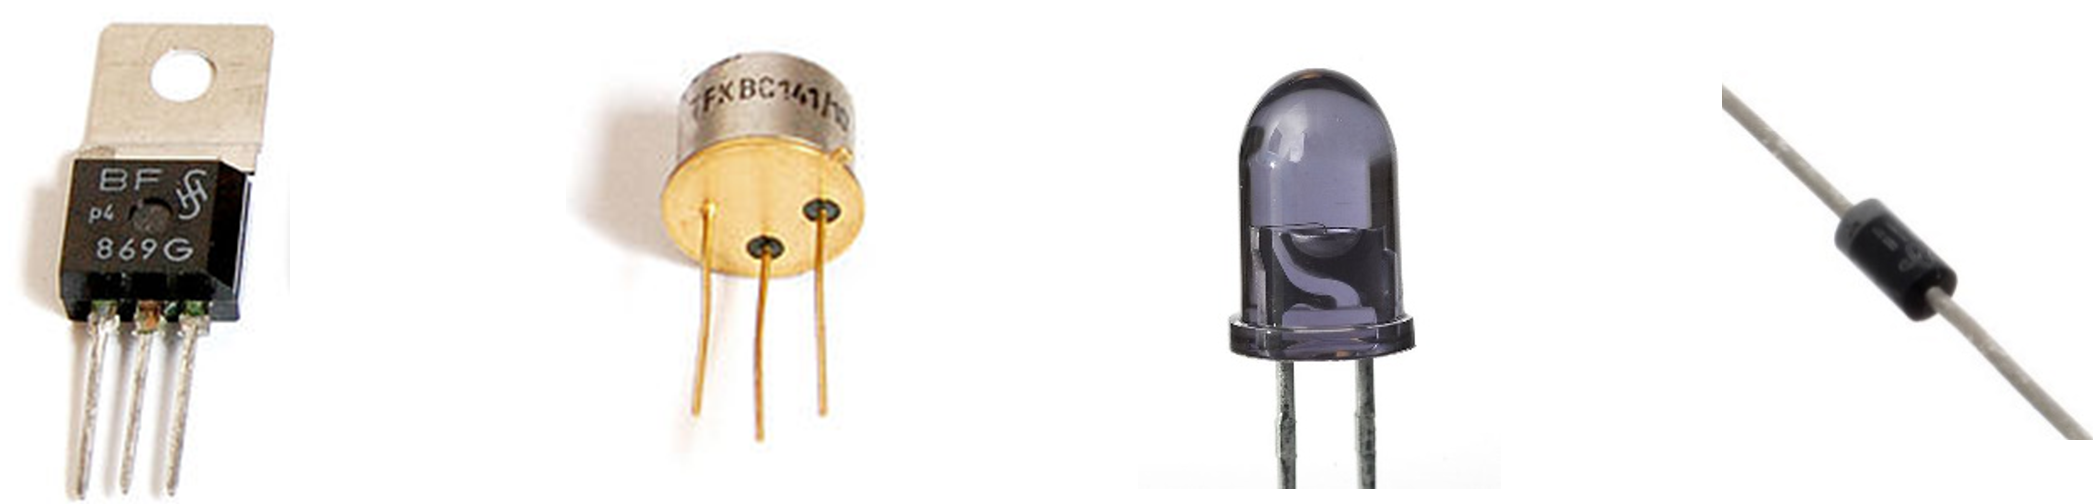
\includegraphics[width=.8\textwidth]{Bilder/kap1/AufnahmenHalbleiterWiki.png}
        %\caption{\textbf{Beispielfotos typischer Halbleiterbauelemente.} V.l.n.r.: Feldeffekttransistor, Bipolartransistor, Leuchtdiode, Diode.}  
        %\label{fig:BeispielfotosVerbreiteterHalbleiterbauelemente}
    \end{figure}
     }
    \speech{Einführung}{2}{Zum Einstieg sehen wir hier eine Auswahl typischer Halbleiterbauelemente.
    Von links nach rechts: ein Feldeffekttransistor, ein Bipolartransistor, eine Leuchtdiode und eine klassische Diode.
    Diese Bauelemente stecken in nahezu jedem elektronischen Gerät - und basieren alle auf denselben physikalischen Prinzipien, die wir uns jetzt nach und nach anschauen.}
\end{frame}

\begin{frame}
\b{\fta{Einführung}
\begin{itemize}
    \item Halbleiterbauelemente sind zentral für die Funktion zahlreicher elektronischer Geräte wie Computer, Mobiltelefone und Solarzellen.
    \item Sie basieren auf Materialien, die weder gute Leiter noch gute Isolatoren sind. Ihre Funktionsweise kann mithilfe des Bändermodells erklärt werden.
    \item In diesem Kapitel werden die Grundlagen der Halbleitertechnik erläutert.
\end{itemize}}
\speech{Einführung}{3}{Halbleiter sind die Grundlage moderner Elektronik - vom Smartphone bis zur Solaranlage.
Sie haben eine besondere Eigenschaft: Sie liegen in ihrer Leitfähigkeit genau zwischen Leitern und Isolatoren.
Und wie lässt sich dieses Verhalten erklären?
Mit dem Bändermodell, das uns zeigt, welche Energiezustände Elektronen in einem Material einnehmen dürfen - und welche nicht.}
\end{frame}

%Zusammenhang Bohrsche Atommodell und Bändermodell.
\begin{frame}
\b{\begin{columns}
    \frametitle{Das Bändermodell}
    \column[c]{0.3\textwidth}
    \begin{figure}[H]
        \onslide<1->{
        \begin{minipage}[t]{0.48\textwidth}
            \begin{figure}[H]
                \centering
                \includesvg[width=1\textwidth]{Bilder/kap1/ZusammenhangBohrscheAtommodellundBaendermodell/ZusammenhangBohrscheAtommodellundBaendermodell_1}
            \end{figure}
        \end{minipage}
} \onslide<2->{
        \begin{minipage}[b]{0.48\textwidth}
                \begin{figure}[H]
                \centering
                \includesvg[width=1.1\textwidth]{Bilder/kap1/ZusammenhangBohrscheAtommodellundBaendermodell/ZusammenhangBohrscheAtommodellundBaendermodell_2}
            \end{figure}
        \end{minipage}
}
        %\caption{\textbf{Zusammenhang zwischen dem Bohrschen Atommodell und Bändermodell.} Darstellung des Zusammenhangs 
                %zwischen dem Abstand von Elektronen zum Kern und Höhe des zugehörigen diskreten Energieniveau. Links: Bohrsche 
                %Atommodell eines Si-Atoms. Rechts: Bändermodell eines Si-Atoms mit den möglichen Energieniveaus.}  
        %\label{fig:ZusammenhangBohrschesAtommodellUndBaendermodell}
    \end{figure}
    \column[c]{0.6\textwidth}
        \begin{itemize}
            \onslide<1->{
            \item Das Bändermodell beschreibt die elektronischen Eigenschaften von Festkörpern und ordnet die Energiezustände von Elektronen in Energiebänder.}
            \onslide<2->{
            \item Es hilft, elektrische, optische und magnetische Eigenschaften von Materialien zu verstehen und zu erklären.}
            \onslide<3->{
            \item Das Modell ermöglicht die Erklärung von Leitung, Isolation, Halbleiterverhalten sowie Oberflächen- und Grenzflächenzuständen.}
            \onslide<4->{
            \item In der Abbildung auf der linken Seite ist der Zusammenhang zwischen bohrschem Atommodell und Bändermodell illustriert.}  
        \end{itemize}
    \end{columns}
}
\speech{Das Bändermodell}{1}{Links sehen wir das Bohrsche Atommodell, das du vielleicht noch aus der Schule kennst:
Elektronen kreisen in definierten Bahnen - oder Schalen - um den Atomkern.
Jede dieser Schalen hat ein festes Energieniveau.
Rechts daneben sehen wir die Entsprechung im Bändermodell:
Auch hier geht es um mögliche Energieniveaus - aber jetzt denken wir nicht mehr an einzelne Bahnen, sondern an Energiezonen im Material, die später zu Bändern zusammengefasst werden.}

\end{frame}

%UebergangVonEnergieniveausZuBaendern
\begin{frame}
    \b{
    \frametitle{Das Bändermodell}
    \begin{figure}[H]
        \centering
        \includesvg[width=\textwidth]{Bilder/kap1/UebergangVonEnergieniveausZuBaendern}
        \caption{\textbf{Übergang von Energieniveaus zu Bändern} Zusammenhang zwischen den möglichen Energiezustände in Abhängigkeit zur Anzahl der Atome. V.l.n.r. Energiezustände von Elektronen bei einem Einzelatom, 2 Atomen (Molekül) und einem Festkörper.}  
        %\label{fig:UebergangVonEnergieniveausZuBaendern}
    \end{figure}

    }
    \speech{Das Bändermodell}{2}{Jetzt gehen wir einen Schritt weiter.
    Ein einzelnes Atom hat klar definierte Energieniveaus - das sehen wir links.
    Kommen zwei Atome zusammen, wirken sie elektrisch aufeinander.
    Nach dem Pauli-Prinzip dürfen zwei Elektronen nicht denselben Zustand einnehmen - ihre Energieniveaus verschieben sich also leicht voneinander.
    Je mehr Atome beteiligt sind, desto mehr dieser leicht verschobenen Niveaus entstehen.
    Im Festkörper - ganz rechts - gibt es dann so viele solcher Zustände, dass sie praktisch ein Kontinuum bilden.
    Und dieses Kontinuum nennen wir ein Energieband.}
\end{frame}

%Bändermodell Eines Materials bei 0K
\begin{frame}
    \b{
    \frametitle{Einteilung von Materialien}
    \begin{figure}[H]
        \centering
        \includesvg[width=\textwidth]{Bilder/kap1/BaendermodelleinesMaterialsbei0K}
        \caption{\textbf{Bändermodell eines Materials bei 0 K} Darstellung der Energiebänder mit zugehöriger Beschriftung sowie deren alternativen Bezeichnungen.}  
        %\label{fig:BandermodellEinesMaterialsBei0K}
    \end{figure}
    }
\speech{Einteilung von Materialien}{1}{Was bedeuten jetzt die Begriffe Valenzband, Leitungsband und Bandlücke?
Das Valenzband ist der Bereich, in dem Elektronen noch fest an die Atome gebunden sind - sie tragen also nicht zur elektrischen Leitung bei.
Das Leitungsband dagegen ist der Bereich, in dem sich Elektronen frei durch das Material bewegen können - das ist entscheidend für den Stromfluss.
Und dazwischen liegt oft eine sogenannte Bandlücke - also ein Energiebereich, in dem sich keine Elektronen aufhalten können.
Die Größe dieser Lücke entscheidet darüber, ob ein Material ein Leiter, ein Halbleiter oder ein Isolator ist.}
\end{frame}

%Bändermodell verschiedener Halbleitermaterialien
\begin{frame}
    \b{
    \frametitle{Einteilung von Materialien}
    \begin{figure}[H]
        \centering
        \includesvg[width=\textwidth]{Bilder/kap1/BaendermodellverschiedenerMaterialien}
        \caption{\textbf{Bändermodell verschiedener Halbleitermaterialien} V.l.n.r.: Leiter ohne und mit Überlappung, Halbleiter und Isolator}  
        %\label{fig:BaendermodellVerschiedenerMaterialien}
    \end{figure}
    }
\speech{Einteilung von Materialien}{2}{In der nächsten Abbildung sehen wir, wie sich Materialien anhand ihrer Bandstruktur unterscheiden.
Links: Leiter - hier liegen Valenz- und Leitungsband direkt aneinander oder überlappen sogar.
Elektronen können also ohne großen Energieaufwand ins Leitungsband gelangen - der Strom fließt leicht.
In der Mitte: der Halbleiter - hier gibt es eine kleine Bandlücke, etwa ein Elektronenvolt.
Elektronen brauchen etwas Energie, zum Beispiel durch Erwärmung, um den Sprung ins Leitungsband zu schaffen.
Und ganz rechts: der Isolator - hier ist die Bandlücke sehr groß, typischerweise über 3 Elektronenvolt.
Der Energieaufwand, um ein Elektron ins Leitungsband zu bringen, ist hier so hoch, dass praktisch kein Strom fließt.}
\end{frame}

%Merke
\begin{frame}
    \b{
    \frametitle{Einteilung von Materialien}
    \textbf{Merke:}
    \begin{itemize}
        \onslide<1->{
        \item Ladungsträger können nur definierte Energieniveaus im Festkörper besetzen.
        }
        \onslide<2->{
        \item Bei $T=\mathrm{0\,K}$ ist das Valenzband das höchste besetzte Energieniveau, das darüberliegende Leistungsband beinhaltet keine freien Ladungsträger.
        }
        \onslide<3->{
        \item Materialien können über die Bandlücke Kategorisiert werden. 
        }
    \end{itemize}}
    \speech{Einteilung von Materialien}{3}{Merken wir uns:
    Nur Elektronen im Leitungsband können sich frei durch das Material bewegen - und damit Strom leiten.
    Ob ein Stoff ein Leiter, Halbleiter oder Isolator ist, hängt also direkt von der Größe der Bandlücke ab.
    Ladungsträger können nur definierte Energieniveaus im Festkörper besetzen.
    Bei T = 0 Kelvin ist das Valenzband das höchste besetzte Energieniveau, das darüberliegende Leistungsband beinhaltet keine freien Ladungsträger.
    Materialien können über die Bandlücke Kategorisiert werden}
\end{frame}


%Diamant-Gitterstruktur von Silizium
\begin{frame}
    \b{
    \frametitle{Halbleitermaterialien}
    \begin{figure}[H]
        \centering
        \includesvg[width=0.4\textwidth]{Bilder/kap1/Gitterstrukturen/GitterSi}
        %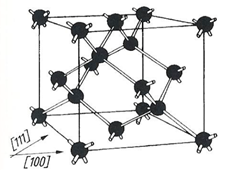
\includegraphics[width=0.5\textwidth]{Bilder/kap1/Diamant-GitterstrukturVonSilizium.png}
        \caption{\textbf{Diamantgitterstruktur von Silizium}}  
        %\label{fig:Diamant-GitterstrukturVonSilizium}
    \end{figure}
    }
    \speech{Halbleitermaterialien}{1}{In diesem Abschnitt schauen wir uns an, wie Halbleitermaterialien aufgebaut sind - und wie man ihre Leitfähigkeit gezielt beeinflussen kann.
    Den Anfang macht das Siliziumgitter.
    Silizium kristallisiert in einer sogenannten Diamantgitterstruktur.
    Das heißt: Jedes Siliziumatom ist tetraedrisch von vier weiteren Atomen umgeben.
    Diese Anordnung sorgt für eine hohe mechanische Stabilität - und gleichzeitig dafür, dass sich Elektronen in alle Richtungen gut bewegen können.
    Ein weiterer Vorteil: Die Struktur ist dreidimensional sehr regelmäßig, was die Halbleitereigenschaften überhaupt erst möglich macht.}
\end{frame}

%Zinkblende-Gitterstruktur von GaAs
\begin{frame}
    \b{
    \frametitle{Halbleitermaterialien}
    \begin{figure}[H]
        \centering
        %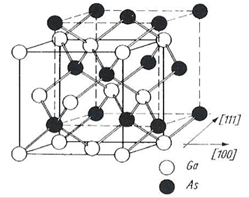
\includegraphics[width=0.5\textwidth]{Bilder/kap1/Zinkblende-GitterstrukturVonGaAs.png}
        \begin{minipage}[c]{0.48\textwidth}
            \centering
            \includesvg[width=0.7\textwidth]{Bilder/kap1/Gitterstrukturen/GitterGaAs_1}
        \end{minipage}
        \begin{minipage}[c]{0.48\textwidth}
            \centering
            \includesvg[width=0.7\textwidth]{Bilder/kap1/Gitterstrukturen/GitterGaAs_2}
        \end{minipage}
        \caption{\textbf{Zinkblende-Gitterstruktur von GaAs}}  
        %\label{fig:Zinkblende-GitterstrukturVonGaAs}
    \end{figure}
    }
    \speech{Halbleitermaterialien}{2}{Ein anderes Beispiel ist Galliumarsenid - ein sogenannter Verbindungshalbleiter.
    Er besteht aus zwei verschiedenen Elementen: Gallium aus der dritten Hauptgruppe und Arsen aus der fünften Hauptgruppe.
    Diese beiden bilden gemeinsam eine Zinkblende-Gitterstruktur - die zwar ähnlich aussieht wie beim Silizium, aber regelmäßig zwischen zwei Atomarten wechselt.
    Diese Kombination sorgt für besondere elektronische Eigenschaften - etwa eine kleinere Bandlücke und gute optische Eigenschaften.
    Deshalb wird Galliumarsenid oft in L E Ds, Laserdioden oder Hochfrequenz-Schaltungen eingesetzt.}
\end{frame}

%Merke
\begin{frame}
    \b{
    \frametitle{Halbleitermaterialien}
    \textbf{Merke:}
    \begin{itemize}
        \onslide<1->{
        \item Silizium ist das am weitesten verbreitete Halbleitermaterial.
        }
        \onslide<2->{
        \item Verbindungshalbleiter bestehen aus zwei Materialen die in bestimmter Kombination Halbleiterverhalten aufweisen.
        }
        \onslide<3->{
        \item Silizium ist aus der IV. Hauptguppe des Periodensystem, Verbindungshalbleiter typischerweise aus der III. und V. Hauptguppe.
        }
    \end{itemize}}
    \speech{Halbleitermaterialien}{3}{Was solltest du dir merken?
Silizium, aus der vierten Hauptgruppe, ist das am häufigsten genutzte Halbleitermaterial - weil es kostengünstig, verfügbar und gut verarbeitbar ist.
Verbindungshalbleiter wie Galliumarsenid bestehen dagegen aus Elementen unterschiedlicher Hauptgruppen, oft der dritten und fünften.
Erst ihre spezielle Kombination ergibt ein stabiles Gitter mit Halbleitereigenschaften.}
\end{frame}

%Tabelle Halbleiter Folie 1
\begin{frame}
    \b{
        \frametitle{Halbleitermaterialien}
        \begin{table}[H]
            \centering 
            \begin{tabular}{|p{1.7cm}|p{1.2cm}|p{2cm}|p{2.2cm}|p{2.2cm}|p{2.3cm}|}
                \hline
                \textbf{Material} & \textbf{Band- \newline lücke \newline (eV)} & \textbf{Ladungs- \newline trägerdichte \newline (cm$^{-3}$)} & \textbf{Elektronen- \newline beweglichkeit \newline (cm$^2$/Vs)} & \textbf{Löcher- \newline beweglichkeit \newline (cm$^2$/Vs)} & \textbf{Anwendungen}\\
                \hline
                Si  & 1,1 & $10^{10} - 10^{15}$ & 1500 & 450 & Mikrochips, \newline Solarzellen, Sensoren \\
                \hline
                Ge & 0,7 & $10^{13} - 20^{19}$ & 3900 & 1900 & Transistoren, \newline Infarot-Detektoren \\
                \hline
                GaAs & 1,43 & $10^6 - 10^8$ & 8500 & 400 & Hochfrequenz- schaltungen, LEDs, Laserdioden \\
                \hline
                \end{tabular}
                \caption{Eigenschaften verschiedener Halbleitermaterialien}
                %\label{tab:EigenschaftenVerschiedenerHalbleitermaterialien}
        \end{table}
    }

    %Gesprochener Text:
    %%
\end{frame}

%Tabelle Halbleiter Folie 1
\begin{frame}
    \b{
        \frametitle{Halbleitermaterialien}
        \begin{table}[H]
            \centering 
            \begin{tabular}{|p{1.7cm}|p{1.2cm}|p{2cm}|p{2.2cm}|p{2.2cm}|p{2.3cm}|}
                \hline
                \textbf{Material} & \textbf{Band- \newline lücke \newline (eV)} & \textbf{Ladungs- \newline trägerdichte \newline (cm$^{-3}$)} & \textbf{Elektronen- \newline beweglichkeit \newline (cm$^2$/Vs)} & \textbf{Löcher- \newline beweglichkeit \newline (cm$^2$/Vs)} & \textbf{Anwendungen}\\
                \hline
                InP & 1,35 & $10^{16} - 10^{17}$ & 5000 - 7000 & 200 - 400 & Optoelektronik, \newline Solarzellen \\
                \hline 
                GaN & 3,4 & $10^{13} - 10^{17}$ & 1000 - 2000 & 50- 200 & Leistungs- \newline elektronik, LED-Beleuchtung, Displays \\
                \hline
                SiC & 3,0 & $10^{12} - 10^{16}$ & 800 - 1200 & 200 - 400 & Leistungs- \newline eletronik, \newline Hochtemperatur- \newline anwendung \\ 
                \hline
                \end{tabular}
                \caption{Eigenschaften verschiedener Halbleitermaterialien}
                %\label{tab:EigenschaftenVerschiedenerHalbleitermaterialien}
        \end{table}
    }
    \speech{Halbleitermaterialien}{4}{Diese Tabellen geben dir einen Überblick über verschiedene Halbleitermaterialien - mit ihren physikalischen Eigenschaften und typischen Anwendungen.
    Wir gehen hier nicht auf jede Zahl ein, aber ein paar Punkte stechen heraus:

    Silizium mit eins Komma eins Elektronenvolt Bandlücke ist der Standard für Mikroelektronik - universell einsetzbar.

    Galliumarsenid hat eine hohe Elektronenbeweglichkeit - deshalb ideal für hohe Frequenzen.

    Gallium-Nitrid und Siliziumcarbid haben eine sehr große Bandlücke - das macht sie perfekt für die Leistungselektronik oder Anwendungen mit hoher Temperatur oder Spannung.

    Wichtig: Je nach Anwendung spielt nicht nur die Bandlücke eine Rolle, sondern auch, wie gut sich Elektronen und sogenannte Löcher im Material bewegen können.}
    

    %Gesprochener Text:
    %%
\end{frame}

%Gitterstruktur und Bändermodell von Si - Abbildung 8
\begin{frame}
    \b{
    \frametitle{Ladungsträgertransport}
    \onslide<1->{
    \begin{minipage}[t]{0.48\textwidth}
        \begin{figure}[H]
            \centering
            \includesvg[width=\textwidth]{Bilder/kap1/GitterstrukturUndBaendermodellVonSi/GitterstrukturUndBaendermodellVonSi_1}
            \caption{\textbf{Gitterstruktur und Bändermodell von Si} reines Silizium bei T $=$ 0 K}  
            \label{fig:GitterstrukturUndBaendermodellVonSi-1}
        \end{figure}
    \end{minipage}
    }
    \onslide<2->{
    \begin{minipage}[t]{0.48\textwidth}
        \begin{figure}[H]
            \centering
            \includesvg[width=\textwidth]{Bilder/kap1/GitterstrukturUndBaendermodellVonSi/GitterstrukturUndBaendermodellVonSi_2}
            \caption{\textbf{Gitterstruktur und Bändermodell von Si} reines Silizium bei T $>$ 0 K}  
            \label{fig:GitterstrukturUndBaendermodellVonSi-2}
        \end{figure}
    \end{minipage}
    }
    }
    \speech{Ladungsträgertransport}{1}{Und wie kommt Bewegung in die Sache?
    Schauen wir uns das Verhalten von reinem Silizium bei verschiedenen Temperaturen an.
    Links: Bei 0 Kelvin ist das Valenzband voll, das Leitungsband leer - das heißt: Keine freien Ladungsträger, kein Stromfluss.
    Rechts: Steigt die Temperatur, erhalten manche Elektronen genug Energie, um in das Leitungsband zu springen.
    Dort sind sie frei beweglich - und zurück bleibt ein Loch im Valenzband, das ebenfalls als positiver Ladungsträger wirkt.
    So entsteht ein Strom - ganz ohne zusätzliche Dotierung.}
\end{frame}

%Gitterstruktur und Bändermodell von n-dotiertem Si - Abbildung 9
\begin{frame}
    \b{\frametitle{Ladungsträgertransport}
    \onslide<1->{
        \begin{minipage}[t]{0.48\textwidth}
            \begin{figure}[H]
                \centering
                \includesvg[width=\textwidth]{Bilder/kap1/GitterstrukturUndBaendermodellVonN-dotiertesSi/GitterstrukturUndBaendermodellVonN-dotiertesSi_1}
                \caption{\textbf{Gitterstruktur und Bändermodell von n-dotiertem Si} n-dotierts Silizium bei T $=$ 0 K.}  
                \label{fig:GitterstrukturUndBaendermodellVonN-DotiertesSi-1}
            \end{figure}
        \end{minipage}
    }
    \onslide<2->{
        \begin{minipage}[t]{0.48\textwidth}
            \begin{figure}[H]
                \centering
                \includesvg[width=\textwidth]{Bilder/kap1/GitterstrukturUndBaendermodellVonN-dotiertesSi/GitterstrukturUndBaendermodellVonN-dotiertesSi_2}
                \caption{\textbf{Gitterstruktur und Bändermodell von n-dotiertem Si} n-dotierts Silizium bei T $>$ 0 K.}  
                \label{fig:GitterstrukturUndBaendermodellVonN-DotiertesSi-2}
            \end{figure}
        \end{minipage}
    }
    }
    \speech{Ladungsträgertransport}{2}{Noch effektiver wird es durch Dotierung.
    Bei der sogenannten n-Dotierung wird zum Beispiel Phosphor eingebracht - ein Element mit fünf Valenzelektronen, eines mehr als Silizium.
    Dieses zusätzliche Elektron ist nur locker gebunden und sitzt in einem Donator-Niveau, knapp unter dem Leitungsband.
    Links: Bei 0 Kelvin bleibt es noch dort - aber rechts sehen wir: Schon bei leicht erhöhter Temperatur kann es ins Leitungsband springen.
    Damit steht sofort ein freies Elektron für den Stromtransport zur Verfügung.
    Durch diese gezielte Veränderung steigt die Leitfähigkeit deutlich.}
\end{frame}

%Gitterstruktur und Bändermodell von p-dotiertem Si
\begin{frame}
    \b{\frametitle{Ladungsträgertransport}
    \onslide<1->{
    \begin{minipage}[t]{0.48\textwidth}
        \begin{figure}[H]
            \centering
            \includesvg[width=\textwidth]{Bilder/kap1/GitterstrukturUndBaendermodellVonP-dotiertesSi/GitterstrukturUndBaendermodellVonP-dotiertesSi_1}
            \caption{\textbf{Gitterstruktur und Bändermodell von p-dotiertem Si} p-dotierts Silizium bei T $=$ 0 K.}  
            \label{fig:GitterstrukturUndBaendermodellVonP-DotiertesSi-1}
        \end{figure}
    \end{minipage}
    }
    \onslide<2->{
    \begin{minipage}[t]{0.48\textwidth}
        \begin{figure}[H]
            \centering
            \includesvg[width=\textwidth]{Bilder/kap1/GitterstrukturUndBaendermodellVonP-dotiertesSi/GitterstrukturUndBaendermodellVonP-dotiertesSi_2}
            \caption{\textbf{Gitterstruktur und Bändermodell von p-dotiertem Si} p-dotierts Silizium bei T $>$ 0 K.}  
            \label{fig:GitterstrukturUndBaendermodellVonP-DotiertesSi-2}
        \end{figure}
    \end{minipage}
    }
    }
    \speech{Ladungsträgertransport}{3}{Bei der p-Dotierung funktioniert es umgekehrt.
    Hier wird etwa Bor eingebracht - das hat nur drei Valenzelektronen.
    Dadurch fehlt ein Elektron für die Bindung - es entsteht ein sogenanntes Loch, also ein leerer Platz im Valenzband.
    Links: Bei 0 Kelvin bleibt das System unbewegt.
    Rechts: Bei höherer Temperatur kann ein Elektron aus der Umgebung in dieses Loch springen.
    Zurück bleibt - wieder - ein Loch, das sich durch das Material bewegen kann und den Stromtransport in positiver Richtung ermöglicht.}
\end{frame}

%Merke
\begin{frame}
    \b{
    \frametitle{Ladungsträgertransport}
    \textbf{Merke:}
    \begin{itemize}
        \onslide<1->{
        \item Durch thermische Anregung können freie Elektronen entstehen, die zum Ladungsträgertransport beitragen. 
        } \onslide<2->{
        \item Dotierung ist das gezielte Einbringen von Fremdatomen mit oder weniger Valenzelektronen als das Ausgangsmaterial.
        } \onslide<3->{
        \item Für n-Dotierung kann Phosphor und für p-Dotierung Bor genutzt werden.
        }
    \end{itemize}}
    \speech{Ladungsträgertransport}{4}{Zusammengefasst:

    Temperatur kann Elektronen anregen - aber noch viel gezielter funktioniert das durch Dotierung.

    Dabei bringt man Atome mit mehr oder weniger Valenzelektronen ins Gitter ein.

    Für n-Dotierung nimmt man zum Beispiel Phosphor, für p-Dotierung Bor.
    So lässt sich die elektrische Leitfähigkeit von Halbleitern ganz gezielt einstellen.}
\end{frame}

%Driftstrom Innerhalb Eines Halbleiters
\begin{frame}
    \b{
    \frametitle{Ladungsträgertransport}
    \begin{figure}[H]
        \centering
        \includesvg[width=0.5\textwidth]{Bilder/kap1/DriftstromInnerhalbEinesHalbleiters}
        \caption{\textbf{Driftstrom innerhalb eines Halbleiters}}  
        %\label{fig:DriftstromInnerhalbEinesHalbleiters}
    \end{figure}
    }
    \speech{Ladungsträgertransport}{5}{In diesem Video schauen wir uns an, wie sich Ladungsträger in Halbleitern bewegen - und was im sogenannten pn-Übergang passiert.
    Fangen wir mit dem Driftstrom an.
    Wenn wir ein elektrisches Feld anlegen, spüren die freien Ladungsträger im Halbleiter - also Elektronen und Löcher - eine Kraft.
    Elektronen driften dann zur positiven Elektrode, Löcher in die entgegengesetzte Richtung.
    In der Abbildung siehst du: Die Bewegung hängt von der Stärke des Feldes und der Beweglichkeit der Teilchen ab.
    Aber: Das ist nur ein Teil der Geschichte.}
\end{frame}

%Diffusions Innerhalb Eines Halbleiters
\begin{frame}
    \b{
    \frametitle{Ladungsträgertransport}
    \begin{figure}[H]
        \centering
        \includesvg[width=0.8\textwidth]{Bilder/kap1/DiffusionsstromInnerhalbEinesHalbleiters}
        \caption{\textbf{Diffusionsstrom innerhalb eines Halbleiters}}  
        %\label{fig:DiffusionsstromInnerhalbEinesHalbleiters}
    \end{figure}
    }
    \speech{Ladungsträgertransport}{6}{Der zweite wichtige Stromanteil ist der Diffusionsstrom.
    Er entsteht ganz ohne äußeres Feld - nämlich dann, wenn es einen Konzentrationsunterschied gibt.
    Freie Elektronen bewegen sich von Bereichen mit hoher Konzentration zu Bereichen mit niedriger - genauso wie bei der Diffusion von Tinte in Wasser.
    In einem n-dotierten Material bedeutet das: Elektronen wandern dorthin, wo es weniger von ihnen gibt - das ist der Diffusionsstrom.
    Und für Löcher im p-Material gilt genau das Gleiche - nur eben umgekehrt.}
\end{frame}

%Einfluss von Spannungen auf Halbleiter
\begin{frame}
    \b{
    \frametitle{Ladungsträgertransport}
    \begin{figure}[H]
        \centering
        \includesvg[width=0.8\textwidth]{Bilder/kap1/EinflussvonSpannungenaufHalbleiter}
        \caption{\textbf{Einfluss von Spannungen auf Halbleiter}}  
        %\label{fig:EinflussVonSpannungenAufHalbleiter}
    \end{figure}
    }
    \speech{Ladungsträgertransport}{7}{Und was passiert, wenn wir eine Spannung anlegen?
    Dann verschieben sich die Energiebänder im Halbleiter.
    Ohne Spannung - links in der Abbildung - sind die Bänder horizontal, es fließt kein Strom.
    Mit Spannung - rechts - entsteht eine Schräglage der Bänder:
    Elektronen streben von hoher zu niedriger Energie - es kommt zum Stromfluss.
    Auch hier wirken Drift und Diffusion wieder zusammen.}
\end{frame}

%Merke
\begin{frame}
    \b{
    \frametitle{Ladungsträgertransport}
    \textbf{Merke:}
    \begin{itemize}
        \onslide<1->{
        \item Driftstrom ist der Ladungsträgertransport auf Grund eines elektrischen Feldes.
        } \onslide<2->{
        \item Diffusionsstrom ist die Bewegung von Ladungsträgern auf Grund eines Konzentrationsunterschiedes.
        } \onslide<3->{
        \item Drift- und Diffusionsstrom ergeben zusammen den Gesamtstrom.
        } \onslide<4->{
        \item Eine externe Spannung führt zu einer Verschiebung des Bändermodells. 
        }
    \end{itemize}}
    \speech{Ladungsträgertransport}{8}{Fassen wir kurz zusammen:

    Driftstrom entsteht durch ein elektrisches Feld,
    Diffusionsstrom durch Konzentrationsunterschiede.
    Beide zusammen ergeben den Gesamtstrom.
    Und: Eine angelegte Spannung verändert das Bändermodell - das ist wichtig für das Verhalten im nächsten Teil.}
\end{frame}

\begin{frame}
    \b{
    \frametitle{pn-Übergang}
    \begin{figure}[H]
        \centering
        \includesvg[width=\textwidth]{Bilder/kap1/FolienVorgaengeInnerhalbeinesPNUebergangs1}
        \caption{\textbf{Vorgänge innerhalb eines pn-Übergangs.}}  
        %\label{fig:VorgaengeInnerhalbEinesPn-Uebergangs1}  
    \end{figure}
    }
    \speech{pn-Übergang}{1}{Jetzt kommen wir zum pn-Übergang - einem zentralen Baustein vieler Bauelemente.
    Er entsteht, wenn ein p-dotierter Halbleiter mit einem n-dotierten verbunden wird.
    Links und rechts sehen wir: In beiden Bereichen gibt es freie Ladungsträger - Elektronen und Löcher.
    Aber in der Mitte, an der Grenze, passiert etwas Interessantes.}
\end{frame}

\begin{frame}
    \b{
    \frametitle{pn-Übergang}
    \begin{figure}[H]
        \centering
        \includesvg[width=0.6\textwidth]{Bilder/kap1/FolienVorgaengeInnerhalbeinesPNUebergangs2}
        \caption{\textbf{Vorgänge innerhalb eines pn-Übergangs.} }  
    \end{figure}
          \begin{itemize}
            \onslide<1->{
        \item Durch die Bindung der Löcher und Elektronen an deren Atome begrenzt den Diffusionsstrom.
            } \onslide<2->{
        \item Der Bereich in der Mitte nennt sich Raumladungszone (RLZ). Dort sind keine freien Ladungsträger, da die Elektronen und Löcher sich gegenseitig neutralisieren.
            } \onslide<3->{
        \item Es entsteht ein elektrisches Feld zwischen den p- und n-dotierten Bereichen.
            }
    \end{itemize}
    }
    \speech{pn-Übergang}{2}{Durch Diffusion wandern Elektronen vom n- ins p-Gebiet, und Löcher vom p- ins n-Gebiet.
    Dabei stoßen sie auf Teilchen mit entgegengesetzter Ladung - und rekombinieren.
    Zurück bleiben ungeladene Atome, die zu geladenen Ionen werden.
    So entsteht in der Mitte eine Zone ohne freie Ladungsträger - die sogenannte Raumladungszone.
    Hier bildet sich ein inneres elektrisches Feld, das eine Art natürliche Sperre bildet.}
\end{frame}

%Vorgänge innerhalb des pn-Übergangs.
\begin{frame}
    \b{
    \frametitle{pn-Übergang}
    \begin{figure}[H]
        \centering
        \includesvg[width=\textwidth]{Bilder/kap1/VorgaengeInnerhalbDesPN-Uebergangs}
        \caption{\textbf{Vorgänge innerhalb des pn-Übergangs.}}  
        %\label{fig:VorgaengeInnerhalbDesPn-Uebergangs}
    \end{figure}
    }
    \speech{pn-Übergang}{3}{In der Raumladungszone wirken jetzt zwei Kräfte gegeneinander:
    Diffusion möchte weiterhin Ladungsträger nach außen treiben,
    das elektrische Feld erzeugt einen Driftstrom in die entgegengesetzte Richtung.
    Im Gleichgewicht ist beides im Gleichgewicht - es fließt kein Strom, obwohl Ladungsträger vorhanden sind.
    Das macht den pn-Übergang so besonders.}
\end{frame}

%Einfluss von Spannungen auf pn-Übergang.
\begin{frame}
    \b{
    \frametitle{pn-Übergang}
    \begin{figure}[H]
        \centering
        \includesvg[width=0.7\textwidth]{Bilder/kap1/EinflussvonSpannungenaufpn-Uebergang}
        \caption{\textbf{Einfluss von Spannungen auf pn-Übergang.} Raumladungszone bei verschiedenen angelegten Spannungen. Links: Spannung in Durchlassrichtung. Rechts: Spannung entgegen der Durchlassrichtung, Sperrrichtung}  
        %\label{fig:EinflussVonSpannungenAufPn-Uebergang}
    \end{figure}
    }
    \speech{pn-Übergang}{4}{Was passiert, wenn wir eine äußere Spannung anlegen?
    Links siehst du den Fall einer Durchlassrichtung:
    Die externe Spannung verringert die Barriere - die Raumladungszone wird schmaler, und Strom kann fließen.
    Rechts: Sperrrichtung - die Spannung verstärkt das innere Feld, die Barriere wächst, und der Stromfluss wird unterdrückt.
    Das ist das Prinzip einer Diode - Strom in eine Richtung ja, in die andere nein.}
\end{frame}

%Merke
\begin{frame}
    \b{
    \frametitle{pn-Übergang}
    \textbf{Merke:}
    \begin{itemize}
        \onslide<1->{
        \item Der pn-Übergang kombiniert eine p- und n-dotierte Halbleiterschicht.
        } \onslide<2->{
        \item Im Übergangsbereich sind keine freien Ladungsträger, der Bereich wird Raumladungszone genannt.
        } \onslide<3->{
        \item In Durchlassrichtung wird die RLZ verkleinert, in Sperrrichtung wird diese vergrößert.  
        }
    \end{itemize}}
    \speech{pn-Übergang}{5}{Was du dir merken solltest:
    Der pn-Übergang ist die Verbindung von p- und n-dotierten Schichten,
    in der Raumladungszone gibt es keine freien Ladungsträger,
    bei Durchlassrichtung wird sie kleiner - bei Sperrrichtung größer.
    Das Verhalten lässt sich durch das Bändermodell und das Wechselspiel aus Drift und Diffusion gut erklären.}
\end{frame}
